%\title{Presentation Template}
\documentclass[10pt]{beamer}

\usetheme[progressbar=frametitle]{metropolis}
\usepackage{appendixnumberbeamer}

\usepackage[compatibility=false]{caption}
\usepackage{subcaption}
\usepackage{csquotes}
\usepackage{booktabs}
\usepackage{hyperref}
\usepackage[scale=2]{ccicons}
\usepackage{tikz}
\usepackage{bm}

\usepackage{caption}
\captionsetup{justification=raggedright,singlelinecheck=false}

\usepackage{sidecap}
\sidecaptionvpos{figure}{c}

\usepackage{fontawesome}

\usepackage{footnpag} %reset footnotes at every page

\makeatother
\renewcommand{\thefootnote}{\ifcase\value{footnote}\or*\or
**\or***\or****\fi}
\makeatletter

\usepackage{xmpmulti}
\usepackage{pgffor}
\usepackage{multimedia}
\usepackage{media9}

\graphicspath{{./img/}}

\usepackage{pgfplots}
\usepgfplotslibrary{dateplot}

\usepackage{xspace}
\newcommand{\themename}{\textbf{\textsc{metropolis}}\xspace}

\definecolor{extralightgray}{gray}{0.85}

\title{Understanding Fraternal Transitions in Individuality}
\subtitle{OEE3 @ ALife 2018}
\date{July 25, 2018}
\author{Matthew Andres Moreno \newline {\faTwitter} @MorenoMatthewA \newline}
\titlegraphic{\vspace{32ex}\hfill
\includegraphics[height=2.5cm]{img/BEACON-logo}}

\usepackage{fix-cm}

\makeatletter\newcommand\HUGE{\@setfontsize\Huge{28}{34}}\makeatother

\begin{document}

\maketitle

% \begin{frame}{Table of contents}
%   \setbeamertemplate{section in toc}[sections numbered]
%   \tableofcontents[hideallsubsections]
% \end{frame}

\section{Background}

\begin{frame}{Why}

\begin{figure}

\includegraphics[width=0.5\textwidth]{blue-brain}
\caption{TODO \cite{trader_2014}}
\end{figure}

\end{frame}


\section{Inducing \& Detecting Fraternal Transitions}

\begin{frame}{Design Objectives}
\Large
expect \textit{detectable} fraternal transition to occur
\begin{itemize}
\item register organisms into explicit, hereditarily-defined cooperating groups
\end{itemize}
\end{frame}

\begin{frame}{Resource Distribution}
\begin{figure}
\begin{columns}
\begin{column}{0.6\textwidth}
  \includegraphics<1>[width=\textwidth]{explanatory_sep/r-2.pdf}%
  \includegraphics<2>[width=\textwidth]{explanatory_sep/r-3.pdf}%
  \includegraphics<3>[width=\textwidth]{explanatory_sep/r-4.pdf}%
  \includegraphics<4>[width=\textwidth]{explanatory_sep/r-5.pdf}%
  \includegraphics<5>[width=\textwidth]{explanatory_sep/r-6.pdf}%
\end{column}
\begin{column}{0.2\textwidth}
\includegraphics<2>[width=\textwidth]{bolt.pdf}%
\end{column}
\end{columns}
\caption{Frame-by-frame animation of a resource wave event.}
\end{figure}
\end{frame}

\begin{frame}{Resource Distribution}
\Large
\textbf{Problem:} how to alert neighbors to available resource?

\pause

\textbf{Solution:} activation-quiescence signaling

\end{frame}

\begin{frame}{Activation-Quiescence Signaling}
\begin{figure}
\begin{columns}
\begin{column}{0.45\textwidth}
  \includegraphics<1>[width=\textwidth]{explanatory_sep/r-2.pdf}%
  \includegraphics<2>[width=\textwidth]{explanatory_sep/r-3.pdf}%
  \includegraphics<3>[width=\textwidth]{explanatory_sep/r-4.pdf}%
  \includegraphics<4>[width=\textwidth]{explanatory_sep/r-5.pdf}%
  \includegraphics<5>[width=\textwidth]{explanatory_sep/r-6.pdf}%
\end{column}
\begin{column}{0.1\textwidth}
\includegraphics<2>[width=\textwidth]{bolt.pdf}%
\end{column}
\begin{column}{0.45\textwidth}

\foreach \n in {1,...,5}{%
  \includegraphics<\n>[width=\textwidth]{explanatory_sep/sig-\n-nohash.pdf}%
}%

\end{column}
\end{columns}

\begin{columns}
\begin{column}{0.45\textwidth}
  \begin{subfigure}[b]{\textwidth}
  \caption{Resource}
  \end{subfigure}
\end{column}

\begin{column}{0.1\textwidth}
\end{column}

\begin{column}{0.45\textwidth}
  \begin{subfigure}[b]{\textwidth}
  \caption{Activation-quiescence signaling}
  \end{subfigure}
\end{column}

\end{columns}


\caption{Frame-by-frame animation of a resource wave event and coupled activation-quiescence signaling.}
\end{figure}
\end{frame}

\begin{frame}{Resource Distribution}
\Large
\textbf{Problem:} how to limit extent of signaling wave?

\normalsize

(i.e., to match limited extent of resource wave)

\Large

\pause

\textbf{Solution:} register cells into explicit cooperating groups called channels

\end{frame}


\begin{frame}{Same-channel Signaling Networks}

\begin{figure}

\begin{columns}
\begin{column}{0.45\textwidth}

  \foreach \n in {1,...,6}{%
  \includegraphics<\n>[width=\textwidth]{explanatory_sep/r-\n.pdf}%
  }%

\end{column}
\begin{column}{0.45\textwidth}

  \foreach \n in {1,...,6}{%
  \includegraphics<\n>[width=\textwidth]{explanatory_sep/s-\n.pdf}%
  }%

\end{column}
\begin{column}{0.1\textwidth}

  \foreach \n in {1,...,6}{%
  \includegraphics<\n>[width=\textwidth]{explanatory_sep/rs-\n.pdf}%
  }%

\end{column}
\end{columns}

\begin{columns}
\begin{column}{0.45\textwidth}
  \begin{subfigure}[b]{\textwidth}
  \caption{Resource}
  \end{subfigure}
\end{column}

\begin{column}{0.45\textwidth}
  \begin{subfigure}[b]{\textwidth}
  \caption{Channel map}
  \end{subfigure}
\end{column}

\begin{column}{0.1\textwidth}
  \begin{subfigure}[b]{\textwidth}
  \end{subfigure}
\end{column}

\end{columns}

\caption{
Frame-by-frame animation of a small same-channel network, activation signal, and resource wave interaction and effect on resource collection.
}

\end{figure}

\end{frame}

\begin{frame}{Same-channel Signaling Networks}

\begin{figure}

\begin{columns}
\begin{column}{0.45\textwidth}

  \foreach \n in {1,...,8}{%
  \includegraphics<\n>[width=\textwidth]{explanatory_sep/r-\n.pdf}%
  }%

\end{column}
\begin{column}{0.45\textwidth}

  \foreach \n in {1,...,8}{%
  \includegraphics<\n>[width=\textwidth]{explanatory_sep/m-\n.pdf}%
  }%

\end{column}
\begin{column}{0.1\textwidth}

  \foreach \n in {1,...,8}{%
  \includegraphics<\n>[width=\textwidth]{explanatory_sep/rm-\n.pdf}%
  }%

\end{column}
\end{columns}

\begin{columns}
\begin{column}{0.45\textwidth}
  \begin{subfigure}[b]{\textwidth}
  \caption{Resource}
  \end{subfigure}
\end{column}

\begin{column}{0.45\textwidth}
  \begin{subfigure}[b]{\textwidth}
  \caption{Channel map}
  \end{subfigure}
\end{column}

\begin{column}{0.1\textwidth}
  \begin{subfigure}[b]{\textwidth}
  \end{subfigure}
\end{column}

\end{columns}

\caption{
Frame-by-frame animation of a medium-sized same-channel network, activation signal, and resource wave interaction and effect on resource collection.
}

\end{figure}

\end{frame}

\begin{frame}{Same-channel Signaling Networks}

\begin{figure}

\begin{columns}
\begin{column}{0.45\textwidth}

  \foreach \n in {1,...,9}{%
  \includegraphics<\n>[width=\textwidth]{explanatory_sep/r-\n.pdf}%
  }%

\end{column}
\begin{column}{0.45\textwidth}

  \foreach \n in {1,...,9}{%
  \includegraphics<\n>[width=\textwidth]{explanatory_sep/l-\n.pdf}%
  }%

\end{column}
\begin{column}{0.1\textwidth}

  \foreach \n in {1,...,9}{%
  \includegraphics<\n>[width=\textwidth]{explanatory_sep/rl-\n.pdf}%
  }%

\end{column}
\end{columns}

\begin{columns}
\begin{column}{0.45\textwidth}
  \begin{subfigure}[b]{\textwidth}
  \caption{Resource}
  \end{subfigure}
\end{column}

\begin{column}{0.45\textwidth}
  \begin{subfigure}[b]{\textwidth}
  \caption{Channel map}
  \end{subfigure}
\end{column}

\begin{column}{0.1\textwidth}
  \begin{subfigure}[b]{\textwidth}
  \end{subfigure}
\end{column}

\end{columns}

\caption{
Frame-by-frame animation of a large same-channel network, activation signal, and resource wave interaction and effect on resource collection.
}

\end{figure}

\end{frame}

\begin{frame}{Same-channel Signaling Networks}

\Large
\textbf{Problem:} how to define same-channel signaling groups?

\pause

\textbf{Solution:} make channel-membership inherited

\normalsize
(with possibility of setting offspring to new channel)

\end{frame}

% \begin{frame}{Channel Inheritance}
%   \vspace{8ex}
%   \begin{figure}
\begin{columns}
  \begin{column}{0.5\textwidth}
    \colorbox{extralightgray}{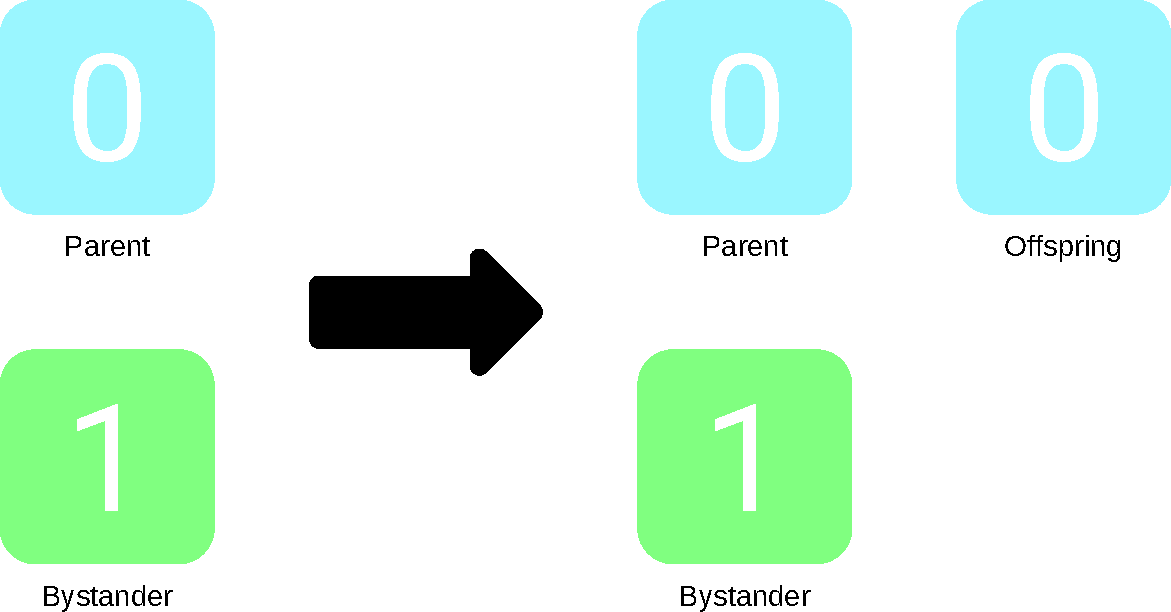
\includegraphics[width=\textwidth]{same_channel_offspring}}
  \end{column}%
  \begin{column}{0.5\textwidth}
    \colorbox{extralightgray}{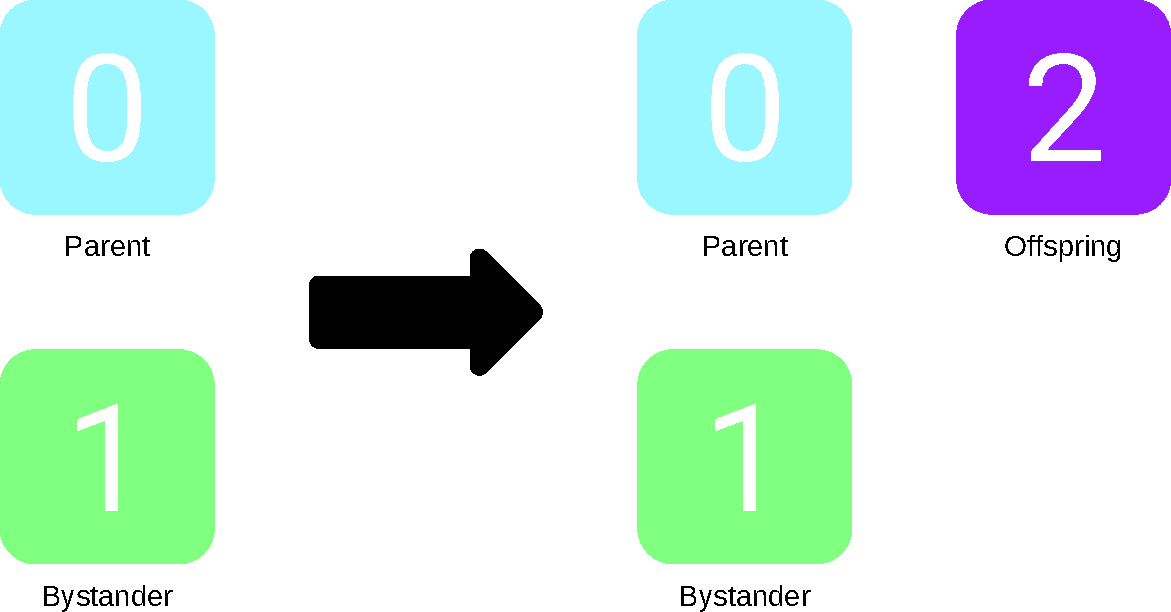
\includegraphics[width=\textwidth]{new_channel_offspring}}
  \end{column}%
\end{columns}%
\begin{columns}
  \begin{column}{0.5\textwidth}
    \begin{subfigure}[b]{\textwidth}
    \caption{Offspring inherits channel ID from parent.}
    \end{subfigure}
  \end{column}%
  \begin{column}{0.5\textwidth}
    \begin{subfigure}[b]{\textwidth}
    \caption{Offspring assigned new, unique channel ID.}
    \end{subfigure}
  \end{column}%
\end{columns}%
\caption{The two possible channel inheritance outcomes.}
\end{figure}

% \end{frame}
%
% \begin{frame}{Excluded Channel Dynamics}
%   \vspace{6.6ex}
%   \begin{figure}
\begin{columns}
  \begin{column}{0.5\textwidth}
\colorbox{extralightgray}{\hspace{0.136\textwidth}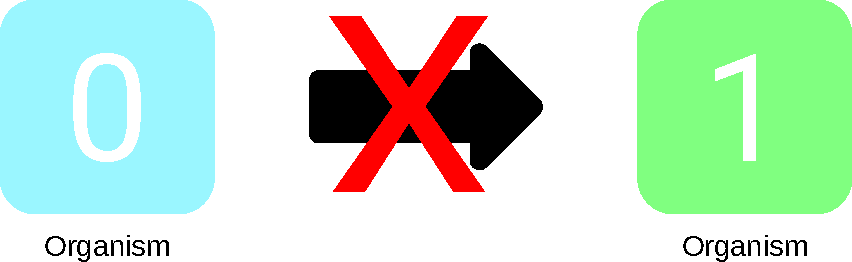
\includegraphics[width=0.728\textwidth,trim= 0 -83 0 -83]{plastic_channel}\hspace{0.136\textwidth}}
  \end{column}%
  \begin{column}{0.5\textwidth}%
\colorbox{extralightgray}{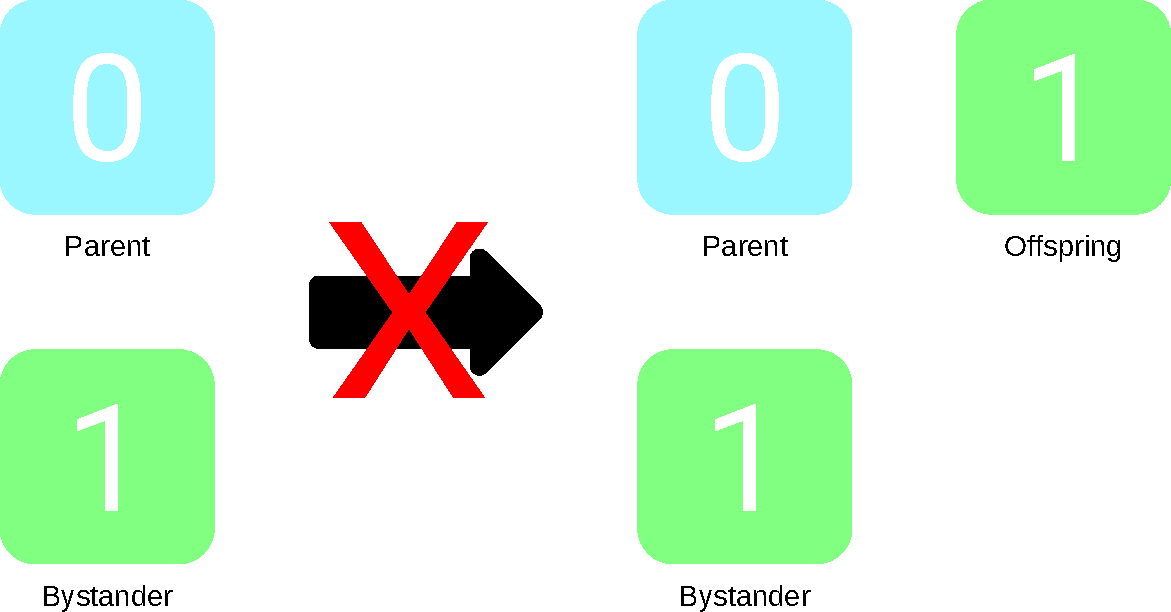
\includegraphics[width=\textwidth]{channel_collision_offspring}}
  \end{column}
\end{columns}%
\begin{columns}
  \begin{column}{0.5\textwidth}
    \begin{subfigure}[b]{\textwidth}
    \caption{during-lifetime channel change}
    \end{subfigure}
  \end{column}
  \begin{column}{0.5\textwidth}
    \begin{subfigure}[b]{\textwidth}
    \caption{non-inherited channel match\footnotemark}
    \end{subfigure}
  \end{column}
\end{columns}
\caption{Illustration of excluded channel dynamics.}
\end{figure}
\footnotetext{infrequent, non-inducible}

% \end{frame}

\begin{frame}{Channels, Signals, \& Resource}
key idea: selection on regulation of same-channel group size \& shape
\pause
\begin{itemize}[<+->]
  \item too small: low resource-collection rate
  \item too big: net negative resource collection due to erroneous activation
  \item coordination task: maintain Goldilocks same-channel network configuration
\end{itemize}

\end{frame}

\begin{frame}{Selection for Same-channel Network Individuality}

\onslide<1->{
\begin{itemize}
\item resource sharing \onslide<9->{$\checkmark$} \onslide<10->{\faSearch}
\item reproductive division of labor \onslide<9->{$\checkmark$} \onslide<11->{\faSearch}
\end{itemize}
}

\begin{figure}
\begin{columns}
\begin{column}{0.5\textwidth}
  \centering
  \onslide<1-7>{
\includegraphics[width=0.7\textwidth]{channelviz/channelviz-clump-crop}}
  \footnotesize
  \begin{itemize}[<+->]
    \item same-channel cells compete, displace one another
    \item clump grows slowly
    \item once full-sized, wastes resource
  \end{itemize}
\end{column}
\begin{column}{0.5\textwidth}
  \centering
  
\includegraphics[width=0.5\textwidth]{channelviz/channelviz-clump2-crop}
  \footnotesize
  \begin{itemize}[<+->]
    \item same-channel cells pool resource, only periphery reproduces
    \item clump grows quickly
    \item once full-sized, accumulates resource wealth
  \end{itemize}
\end{column}
\end{columns}
\caption{A juxtaposition of two (competing) clumps.}
\end{figure}

\end{frame}


\section{Hierarchical Extension}

\begin{frame}{Clumps \& Clumps of Clumps}

\vspace{4ex}

\begin{figure}
\begin{columns}
\begin{column}{0.05\textwidth}
\begin{subfigure}[b]{\textwidth}
\caption{}
\label{fig:natural}
\end{subfigure}
\end{column}
\begin{column}{0.27\textwidth}
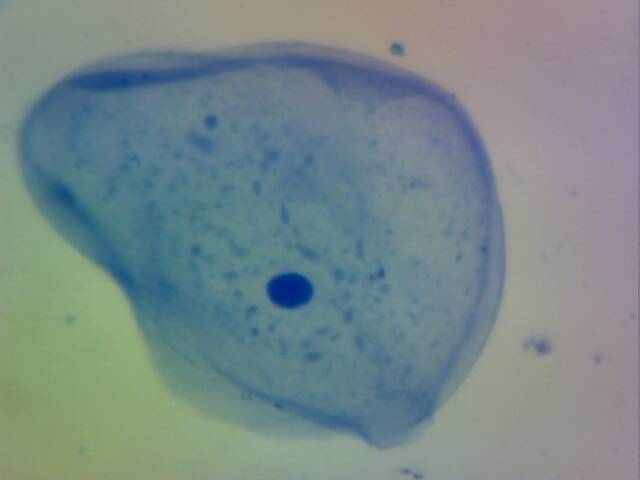
\includegraphics[width=\textwidth]{cheek_cell}
\end{column}
\begin{column}{0.07\textwidth}

\includegraphics[width=\textwidth]{arrow}
\end{column}
\begin{column}{0.27\textwidth}
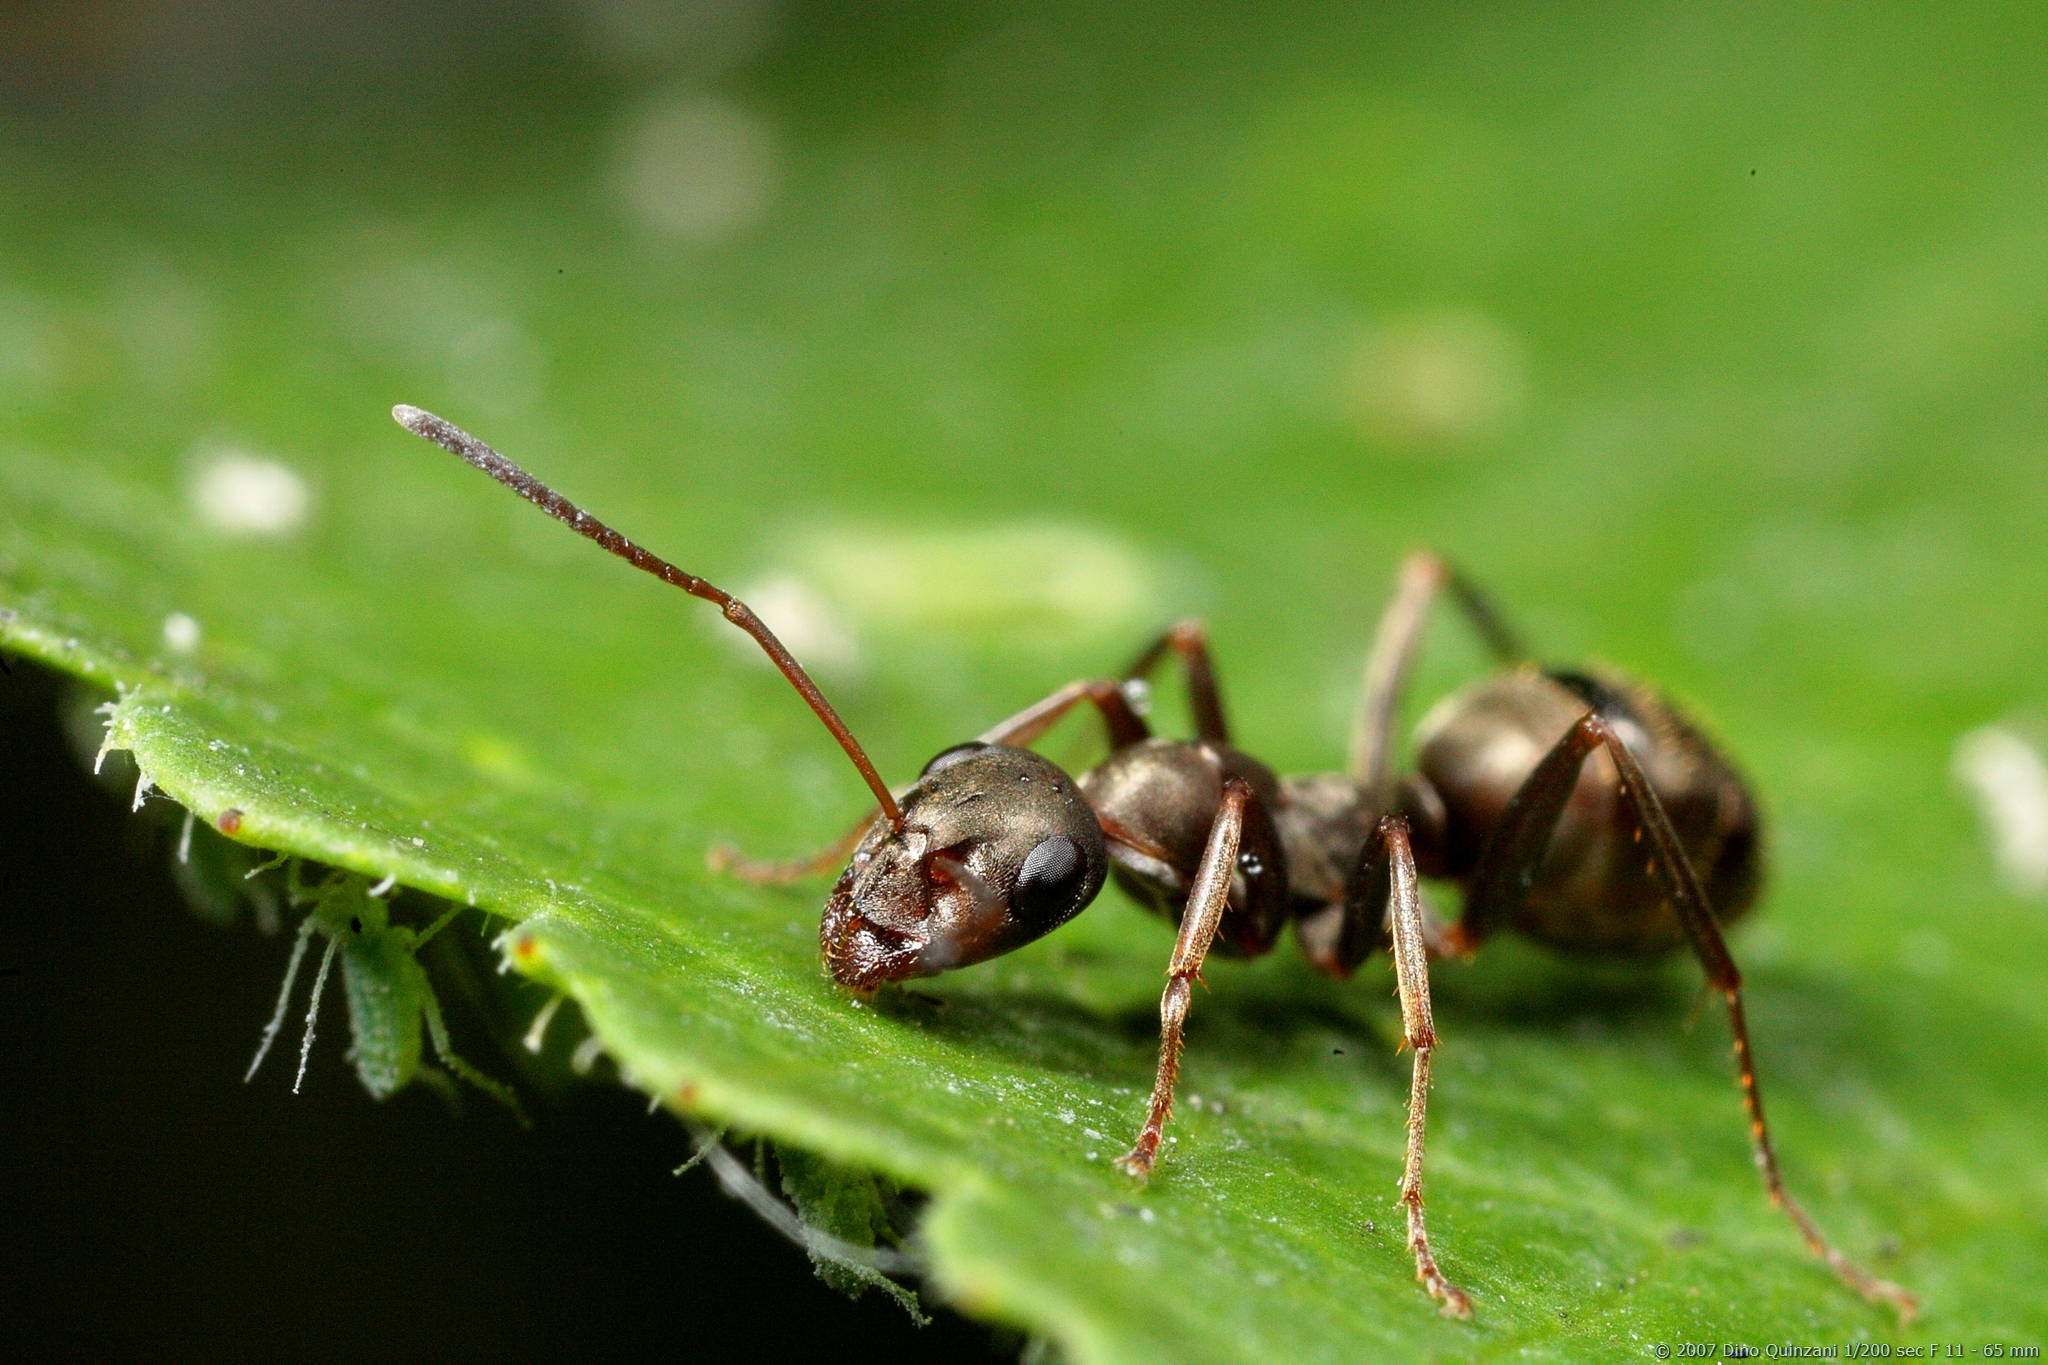
\includegraphics[width=\textwidth]{ant}
\end{column}
\begin{column}{0.07\textwidth}

\includegraphics[width=\textwidth]{arrow}
\end{column}
\begin{column}{0.27\textwidth}
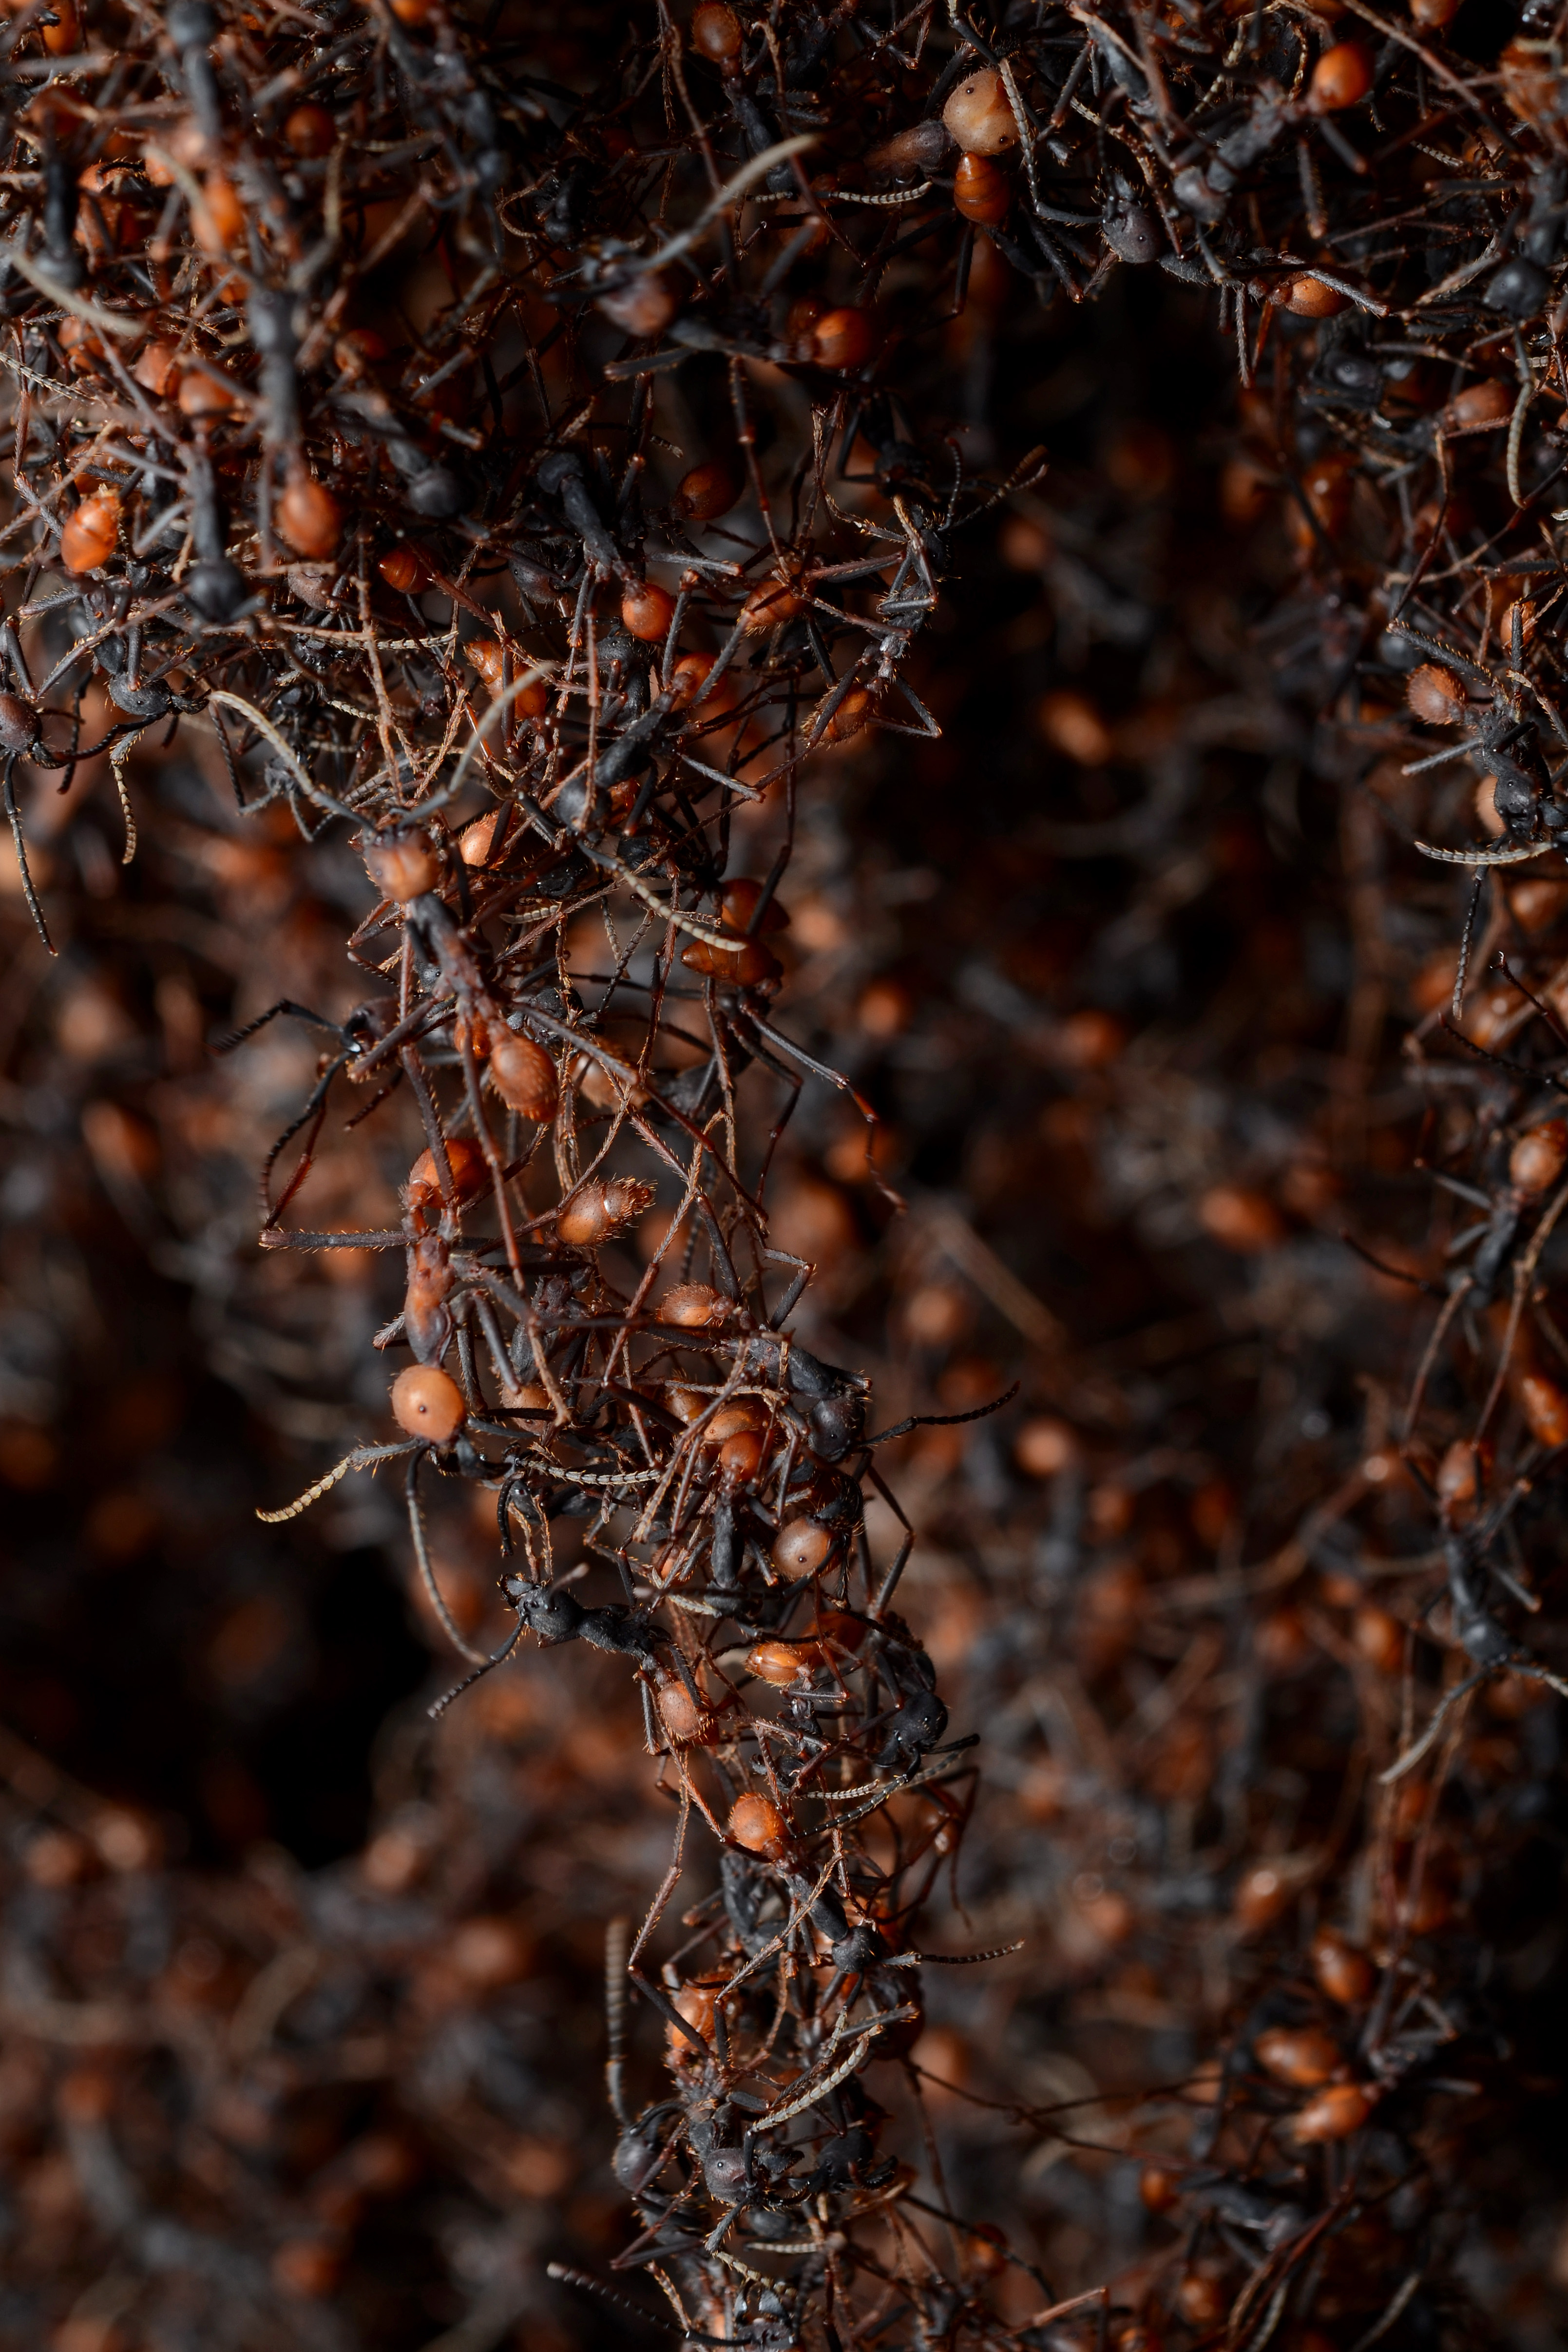
\includegraphics[angle=270, width=\textwidth]{ant_bridge}
\end{column}
\end{columns}
\vspace{1ex}
\begin{columns}
\begin{column}{0.05\textwidth}
\end{column}
\begin{column}{0.27\textwidth}
\centering
cell {\tiny\cite{clare_and_ben_2017}}
\end{column}
\begin{column}{0.07\textwidth}
\end{column}
\begin{column}{0.27\textwidth}
\centering
ant {\tiny\cite{quinzani_2008}}
\end{column}
\begin{column}{0.07\textwidth}
\end{column}
\begin{column}{0.27\textwidth}
\centering
ant colony {\tiny\cite{gallice_2011}}
\end{column}
\end{columns}
\begin{columns}
\begin{column}{0.05\textwidth}
\end{column}
\begin{column}{0.27\textwidth}
\centering
\end{column}
\begin{column}{0.07\textwidth}
\end{column}
\begin{column}{0.27\textwidth}
\centering
(clump)
\end{column}
\begin{column}{0.07\textwidth}
\end{column}
\begin{column}{0.27\textwidth}
\centering
(clump of clumps)
\end{column}
\end{columns}
\vspace{2ex}
\begin{columns}
\begin{column}{0.05\textwidth}
\begin{subfigure}[b]{\textwidth}
\caption{}
\label{fig:simulated}
\end{subfigure}
\end{column}
\begin{column}{0.27\textwidth}

\includegraphics[width=\textwidth]{cell}
\end{column}
\begin{column}{0.07\textwidth}
{\Large$\underset{\phantom{\checkmark}}{\overset{\checkmark}{
\includegraphics[width=\textwidth]{arrow}}}$}
\end{column}
\begin{column}{0.27\textwidth}
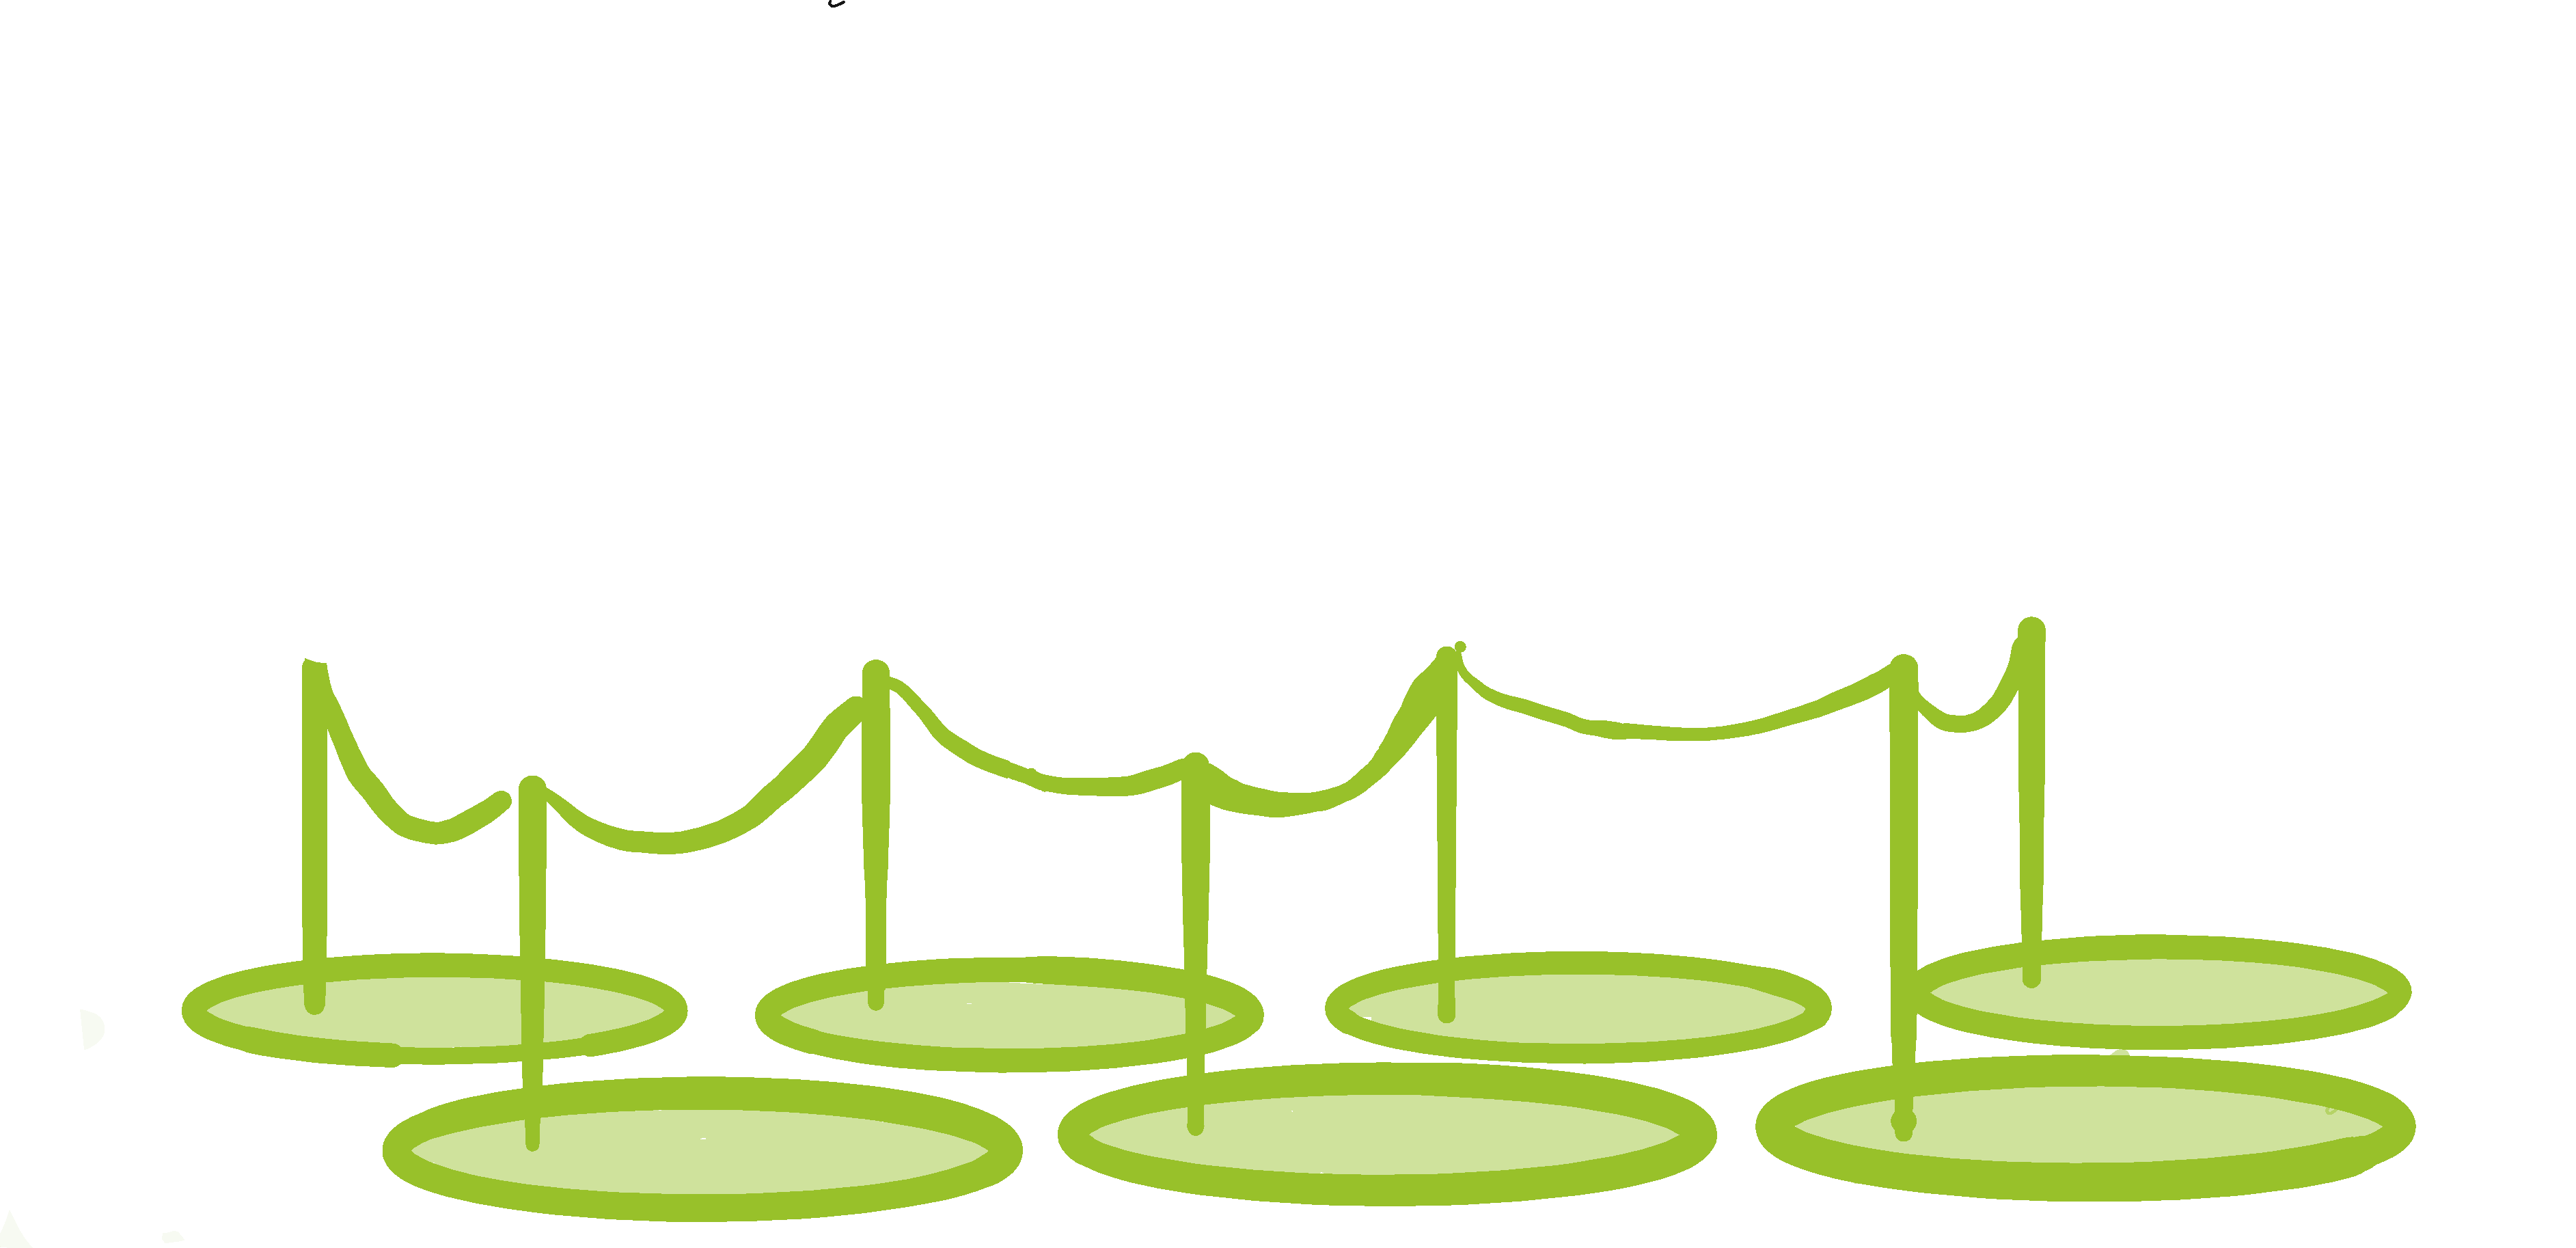
\includegraphics[width=\textwidth]{clump}
\end{column}
\begin{column}{0.07\textwidth}
{\Large$\underset{\phantom{?}}{\overset{\only<1,2>{?}\only<3>{\phantom{?}}}{
\includegraphics[width=\textwidth]{arrow}}}$}
\end{column}
\begin{column}{0.27\textwidth}
\centering
\only<1,2>{\Large ?} \only<3>{\Large \phantom{?}}
\includegraphics[width=\textwidth]<2>{clumps}
\includegraphics[width=\textwidth]<3>{clump_of_clumps}
\end{column}
\end{columns}
\vspace{1ex}
\begin{columns}
\begin{column}{0.05\textwidth}
\end{column}
\begin{column}{0.27\textwidth}
\centering
cell
\end{column}
\begin{column}{0.07\textwidth}
\end{column}
\begin{column}{0.27\textwidth}
\centering
clump
\end{column}
\begin{column}{0.07\textwidth}
\end{column}
\begin{column}{0.27\textwidth}
\centering
\only<3>{\phantom{(}}\only<1,2>{(}clump of clumps\only<1,2>{)}\only<3>{\phantom{)}}
\end{column}
\end{columns}
\vspace{2ex}
\caption{Analogy between (\subref{fig:natural}) natural and (\subref{fig:simulated}) simulated hierarchical fraternal transitions of individuality.}

\end{figure}


\end{frame}


\begin{frame}{Clumps \& Clumps of Clumps}
\begin{figure}
\begin{columns}
  \begin{column}{0.5\textwidth}
    \includegraphics<1>[width=\textwidth]{hsvmap/hsvmap-clump}%
    \includegraphics<2>[width=\textwidth]{hsvmap/hsvmap-clump}%
    \includegraphics<3>[width=\textwidth]{hsvmap/hsvmap-clumpofclumps}%
    \includegraphics<4>[width=\textwidth]{hsvmap/hsvmap-clumpsofclumps}%
  \end{column}
  \begin{column}{0.5\textwidth}
    \includegraphics<1>[width=\textwidth]{channelviz/channelviz-cell}%
    \includegraphics<2>[width=\textwidth]{channelviz/channelviz-clump}%
    \includegraphics<3>[width=\textwidth]{channelviz/channelviz-clumpofclumps}%
    \includegraphics<4>[width=\textwidth]{channelviz/channelviz-clumpsofclumps}%
  \end{column}
\end{columns}
\begin{columns}
  \begin{column}{0.5\textwidth}
    \begin{subfigure}[b]{\textwidth}
    \caption{channel ID HSV key}
    \end{subfigure}
  \end{column}
  \begin{column}{0.5\textwidth}
    \begin{subfigure}[b]{\textwidth}
    \caption{channel map visualization}
    \end{subfigure}
  \end{column}
\end{columns}
\caption{Visualization of hierarchically-nested signaling networks.}
\end{figure}
\end{frame}


\begin{frame}{Signals \& Resource}
  \begin{figure}
\begin{columns}
\begin{column}{0.02\textwidth}
\rotatebox{90}{Level 2}
\end{column}
\begin{column}{0.49\textwidth}
    \centering
    \foreach \n in {1,...,12}{%
    \includegraphics<\n>[width=\textwidth,trim={0 0 0 250},clip]{big_res/frame-\n.png}%
    }%
\end{column}
\begin{column}{0.49\textwidth}
  \centering
  \foreach \n in {1,...,12}{%
  \includegraphics<\n>[width=\textwidth,trim={0 0 0 250},clip]{big_sig/frame-\n.png}%
  }%
\end{column}
\end{columns}%
\vspace{2ex}
\begin{columns}
\begin{column}{0.02\textwidth}
  \rotatebox{90}{Level 1}
\end{column}
\begin{column}{0.49\textwidth}
    \centering
    \foreach \n in {1,...,12}{%
    \includegraphics<\n>[width=\textwidth,trim={0 0 0 250},clip]{small_res/frame-\n.png}%
    }%
\end{column}
\begin{column}{0.49\textwidth}
  \centering
  \foreach \n in {1,...,12}{%
  \includegraphics<\n>[width=\textwidth,trim={0 0 0 250},clip]{small_sig/frame-\n.png}%
  }%
\end{column}
\end{columns}%
\begin{columns}
\begin{column}{0.02\textwidth}
\end{column}
\begin{column}{0.49\textwidth}
\begin{subfigure}[b]{\textwidth}
  \caption{resource}
\end{subfigure}
\end{column}
\begin{column}{0.49\textwidth}
\begin{subfigure}[b]{\textwidth}
\caption{activation-quiescence signals}
\end{subfigure}
\end{column}
\end{columns}
\caption{Co-visualization of same-channel signaling and resource distribution.}
\end{figure}

\end{frame}


\begin{frame}{Clumps of Clumps}
    % \multiinclude[format=png,start=0
    % ,graphics={width=\textwidth}]{multichannel/frame}
\end{frame}

\begin{frame}{Signals \& Resource: Level 2 {\small(Clumps of Clumps)}}
foo
\end{frame}

\begin{frame}{Multichannel Inheritance Outcomes}
  \begin{figure}
  \begin{subfigure}[b]{0.85\textwidth}
    \begin{columns}
    \begin{column}{0.05\textwidth}
      \caption{}~\\\vspace{0ex}~\\
      \label{fig:same_multichannel_offspring}
    \end{column}
    \begin{column}{0.95\textwidth}
      \colorbox{extralightgray}{
\includegraphics[width=\textwidth]{same_multichannel_offspring}}
  \end{column}
\end{columns}
  \end{subfigure}
  \begin{subfigure}[b]{0.85\textwidth}
      \begin{columns}
      \begin{column}{0.05\textwidth}
        \caption{}~\\\vspace{0ex}~\\
        \label{fig:new_lowchannel_offspring}
      \end{column}
      \begin{column}{0.95\textwidth}
        \colorbox{extralightgray}{
\includegraphics[width=\textwidth]{new_lowchannel_offspring}}
\end{column}
\end{columns}
  \end{subfigure}
  \begin{subfigure}[b]{0.85\textwidth}
      \begin{columns}
      \begin{column}{0.05\textwidth}
      \caption{}~\\\vspace{0ex}~\\
      \label{fig:new_highchannel_offspring}
      \end{column}
      \begin{column}{0.95\textwidth}
        \colorbox{extralightgray}{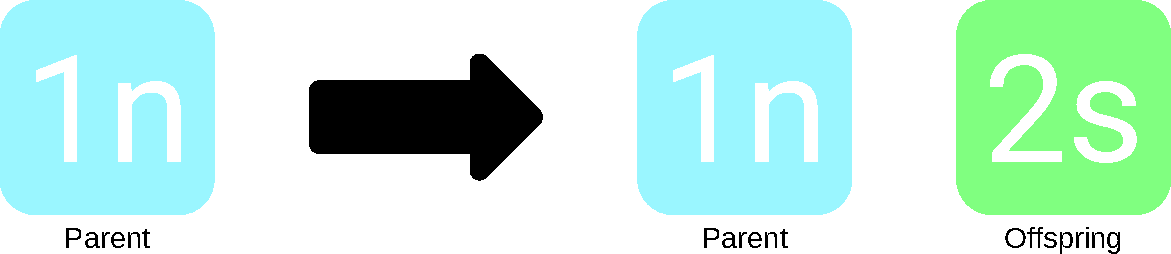
\includegraphics[width=\textwidth]{new_highchannel_offspring}\vspace{-10ex}}
\end{column}
\end{columns}
  \end{subfigure}
  \caption{
  Allowed multichannel inheritance outcomes;
  (\subref{fig:same_multichannel_offspring}) identical level 1 and 2 channels,
  (\subref{fig:new_lowchannel_offspring}) new level 1 channel with identical level 2 channel, and
  (\subref{fig:new_highchannel_offspring}) new level 1 and 2 channels.
  }
\end{figure}

\end{frame}

\begin{frame}{Signals \& Resource: Level 1 {\small(Clumps)} \& Level 2 {\small(Clumps of Clumps)}}%
  foo
\end{frame}


\section{Experiment}

\begin{frame}{Experiment}

Goal: test if DISHTINY scheme selects for higher-order individuality

\end{frame}

\begin{frame}{What's Evolving?}

Manually-designed strategy parameters:
\begin{itemize}
\item Should I reproduce over a neighbor that shares my signaling channel?
\item Should I share resources with my signaling channel network?
\item How big should my signaling channel get before I start making propagules?
\item How much resource should I endow propagules with?
\item Should I attempt an apoptosis response to mutation?
\end{itemize}
\end{frame}

\section{Preliminary Results}
\section{Preliminary\** Results}


\begin{frame}{Outcomes}

Categorized outcomes by resource-sharing of dominant genotype:
\begin{itemize}
\item hog resources to cell (Cell-level individuals) 2
\item share resources with Level 1 same-channel network (Level-one individuals) 16
\item share resources with Level 2 same-channel network (Level-two individuals) 15
\end{itemize}

\end{frame}

\begin{frame}{Outcome: Cell-level Individuality}
\begin{figure}
\begin{columns}
\begin{column}{0.6\textwidth}
% 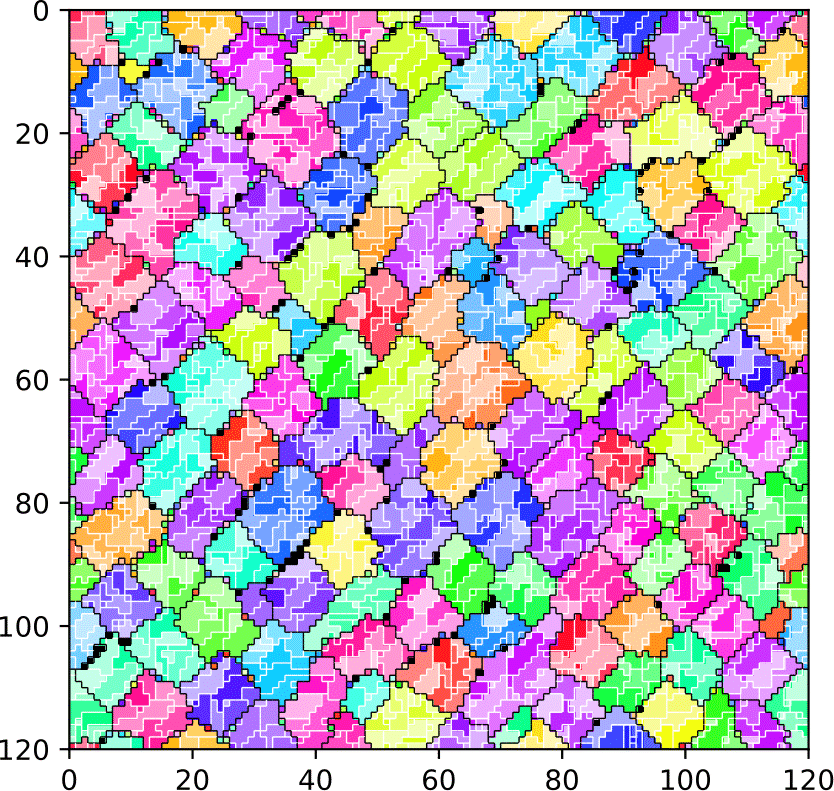
\includegraphics[width=\textwidth]{img/results/ChannelMap_1022_update19500000}
\end{column}
\begin{column}{0.4\textwidth}
\caption{
End state of same-channel signaling networks in simulation where cell-level individuality dominated.
}
\end{column}
\end{columns}
\end{figure}
\end{frame}

\begin{frame}{Outcome: Level-one Individuality}
\begin{figure}
\begin{columns}
\begin{column}{0.6\textwidth}
% 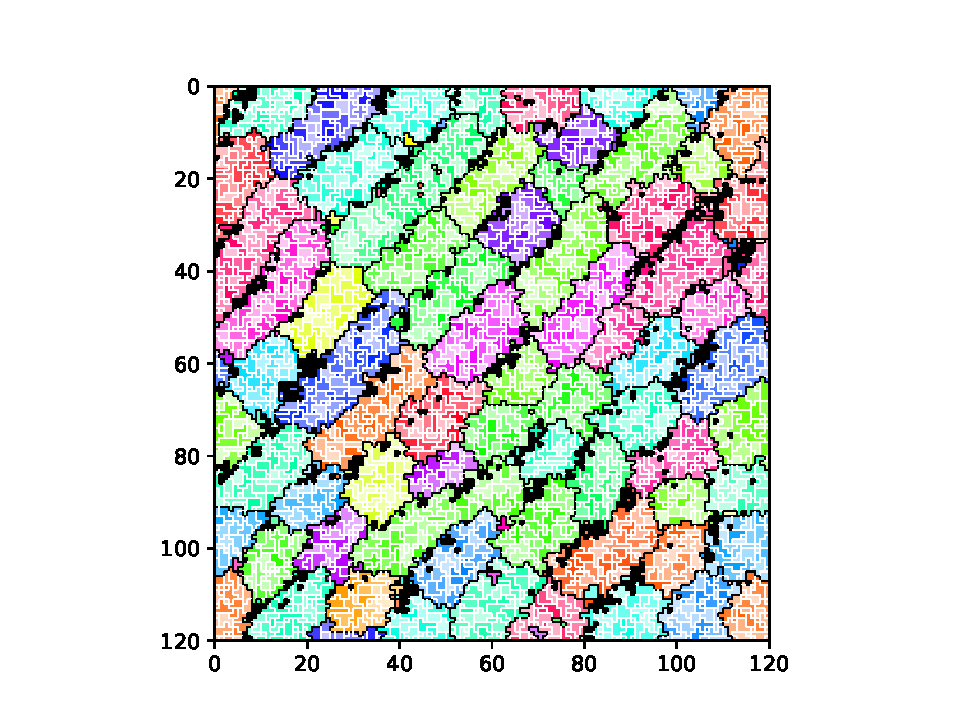
\includegraphics[width=\textwidth]{img/results/ChannelMap_1041_update19500000}
\end{column}
\begin{column}{0.4\textwidth}
\caption{
End state of same-channel signaling networks in simulation where level-one individuality dominated.
}
\end{column}
\end{columns}
\end{figure}
\end{frame}

\begin{frame}{Outcome: Level-two Individuality}
\begin{figure}
\begin{columns}
\begin{column}{0.6\textwidth}
% 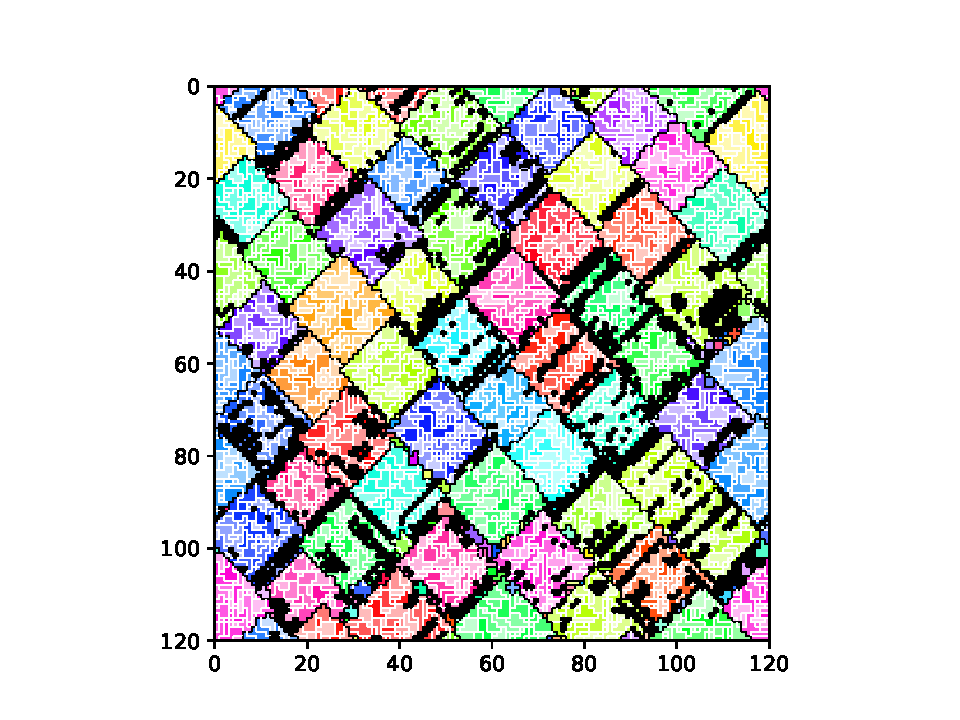
\includegraphics[width=\textwidth]{img/results/ChannelMap_1047_update19500000}
\end{column}
\begin{column}{0.4\textwidth}
\caption{
End state of same-channel signaling networks in simulation where level-two individuality dominated.
}
\end{column}
\end{columns}
\end{figure}
\end{frame}

\begin{frame}{Outcome: Evolution of Level-two Individuality}
\begin{figure}
\begin{columns}
\begin{column}{0.6\textwidth}
% \includegraphics<1>[width=\textwidth]{results/ChannelMap_1011_update0.pdf}%
% \includegraphics<2>[width=\textwidth]{results/ChannelMap_1011_update500000.pdf}%
% \includegraphics<3>[width=\textwidth]{results/ChannelMap_1011_update1000000.pdf}%
% \includegraphics<4>[width=\textwidth]{results/ChannelMap_1011_update2000000.pdf}%
% \includegraphics<5>[width=\textwidth]{results/ChannelMap_1011_update4000000.pdf}%
% \includegraphics<6>[width=\textwidth]{results/ChannelMap_1011_update5000000.pdf}%
% \includegraphics<7>[width=\textwidth]{results/ChannelMap_1011_update7000000.pdf}%
\end{column}
\begin{column}{0.4\textwidth}
\only<1>{Update: 0}%
\only<2>{Update: 500,000}%
\only<3>{Update: 1,000,000}%
\only<4>{Update: 2,000,000}%
\only<5>{Update: 4,000,000}%
\only<6>{Update: 5,000,000}%
\only<7>{Update: 7,000,000}%

\vspace{8ex}

\caption{Channel-map visualization of a simulation where second-level individuality evolved.}
\end{column}
\end{columns}
\end{figure}
\end{frame}

\begin{frame}{Level-one vs. Level-two Relative Fitness}

\begin{figure}
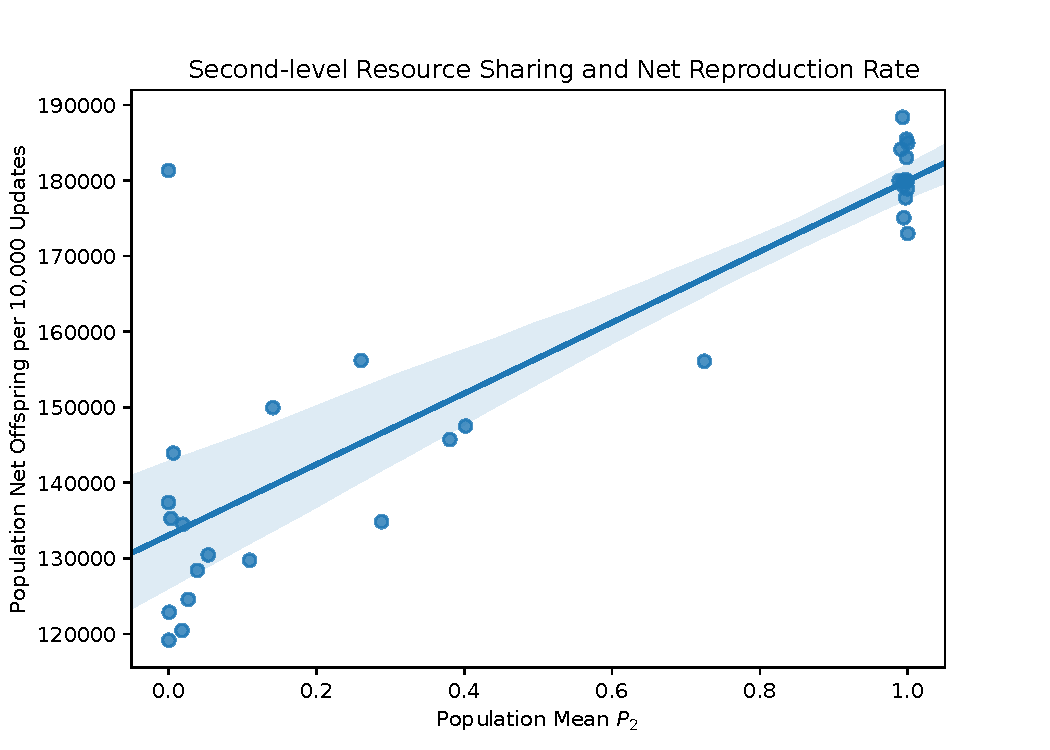
\includegraphics[width=\textwidth]{results/mean_res_pool2_vs_net_reproduction}
\caption{
Correlation plot of population mean $P_2$ (resource-caching strategy) and population net reproduction rate.
A bootstrapped 95\% confidence interval for the fit is shaded.
}
\end{figure}

\end{frame}

\begin{frame}{Level-two Individuals' Apoptosis Response to Mutation}

\begin{figure}
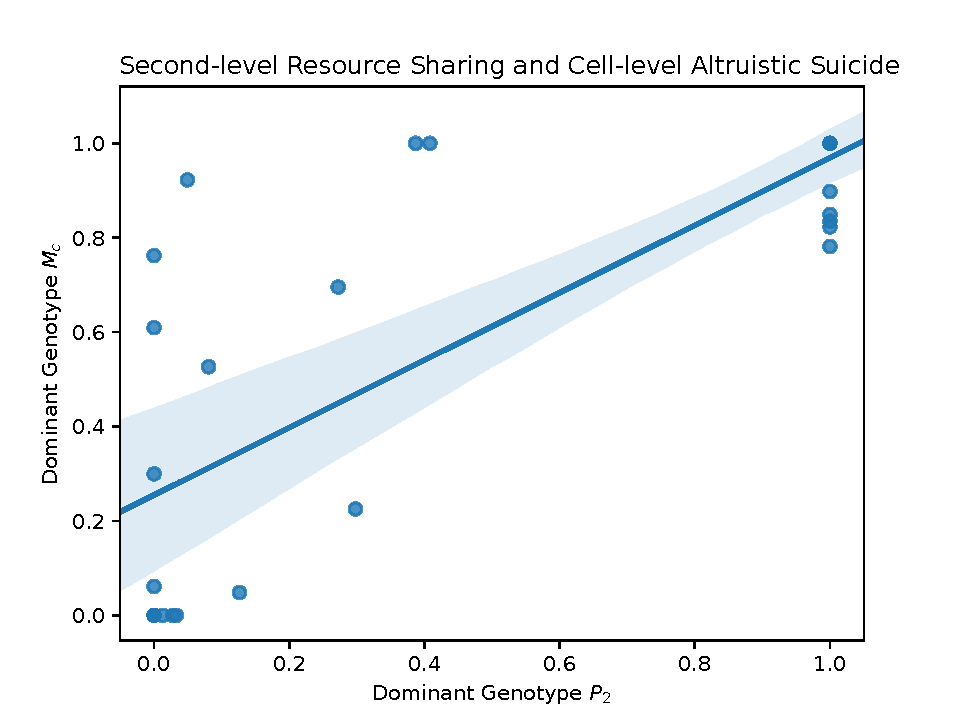
\includegraphics[width=\textwidth]{results/champion_res_pool2_vs_champion_damage_suicide0}
\caption{
Correlation plot of dominant genotype $P_2$ (resource-caching strategy) and dominant genotype $M_{c}$ (apoptosis response to mutation).
A bootstrapped 95\% confidence interval for the fit is shaded.
}
\end{figure}

\end{frame}


\appendix

\begin{frame}{For More Information}

\vspace{1ex}

{\HUGE\url{https://osf.io/ewvg8/}}

\vspace{3ex}

\begin{itemize}
\item live in-browser demo
\item source code
\item data
\item figures and graphics
\item how-to-replicate tutorial
\item publication
\item slides
\item blog article
\end{itemize}

\end{frame}

\begin{frame}{People}

\begin{columns}
\begin{column}{0.25\textwidth}
  \centering
  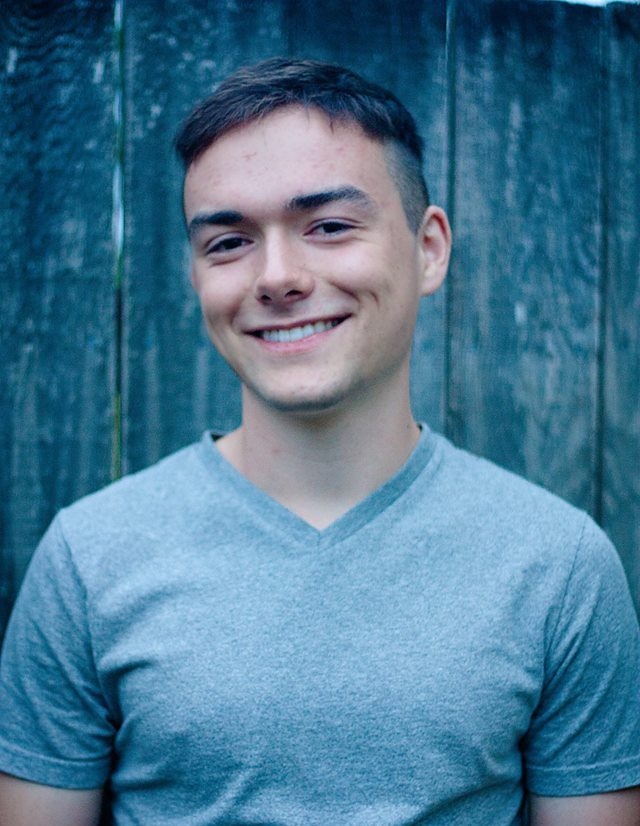
\includegraphics[width=0.7\textwidth]{moreno}
\end{column}
\begin{column}{0.75\textwidth}
  \textbf{Matthew Andres Moreno}

  \href{https://twitter.com/MorenoMatthewA}{{\faTwitter} @MorenoMatthewA}

  \href{https://mmore500.github.io}{{\faGlobe} \texttt{https://mmore500.github.io}}

  \href{mailto: mmore500@msu.edu}{{\faEnvelope} \texttt{mmore500@msu.edu}}

\end{column}
\end{columns}

\vspace{1ex}

\begin{columns}
\begin{column}{0.25\textwidth}
  \centering
  \includegraphics[width=0.7\textwidth]{ofria}
\end{column}

\begin{column}{0.75\textwidth}
  \textbf{Charles Ofria}

  \href{https://twitter.com/CharlesOfria}{{\faTwitter} @CharlesOfria}

  \href{https://ofria.com}{{\faGlobe} \texttt{https://ofria.com}}

  \href{mailto: ofria@msu.edu}{{\faEnvelope} \texttt{ofria@msu.edu}}

\end{column}
\end{columns}
\vfill
\begin{columns}
\begin{column}{0.5\textwidth}
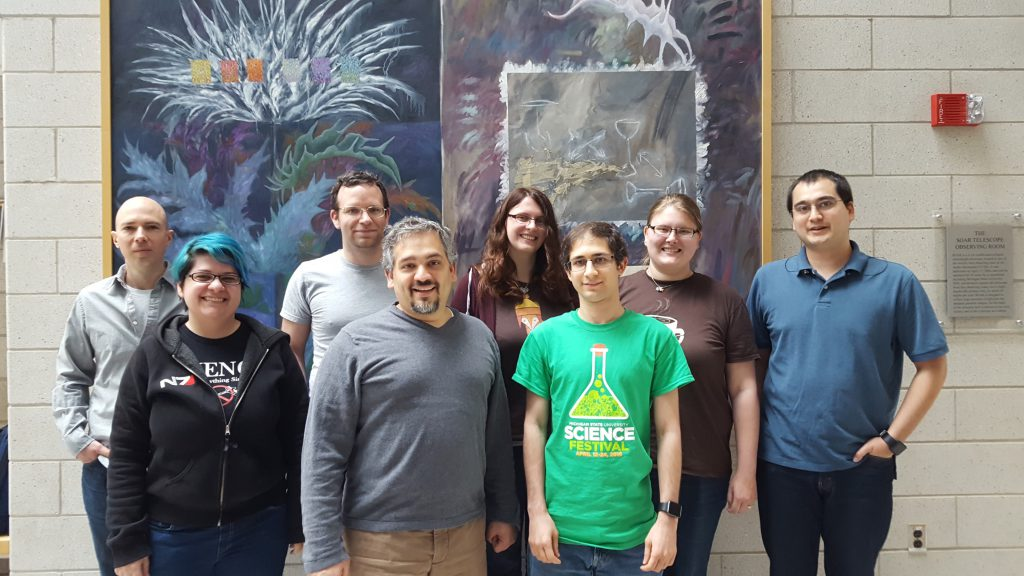
\includegraphics[width=\textwidth, trim={0 0 0 150}, clip]{group_photo}
\end{column}
\begin{column}{0.5\textwidth}

\includegraphics[width=\textwidth]{devolab-logo}
\end{column}
\end{columns}

\end{frame}

\begin{frame}{Acknowledgements}
\begin{itemize}
\item Empirical Library for scientific software development in C++
\item Open Science Framework via the Center for Open Science
\item computational resources via Michigan State University's Institute for Cyber-Enabled Research
\item This research was supported in part by NSF grants DEB-1655715 and DBI-0939454.\footnote[1]{Any opinions, findings, and conclusions or recommendations expressed in this material are those of the author(s) and do not necessarily reflect the views of the National Science Foundation.}
\end{itemize}

\vfill

\newcommand{\innerspacer}{0.07\textwidth}
\newcommand{\content}{0.24\textwidth}
\newcommand{\outerspacer}{0.07\textwidth}

\begin{center}
 \begin{columns}
	\begin{column}{\outerspacer}~\end{column}
	 \begin{column}{\content}
		
\includegraphics[width=\textwidth]{NSF-logo}
 	\end{column}
  \begin{column}{\innerspacer}~\end{column}
	 \begin{column}{\content}
		
\includegraphics[width=\textwidth]{BEACON-logo}
 	\end{column}
  \begin{column}{\innerspacer}~\end{column}
 	\begin{column}{\content}
   
\includegraphics[width=0.75\textwidth]{MSU-helmet}
 	\end{column}
 	\begin{column}{\outerspacer}~\end{column}
 \end{columns}
\end{center}

\end{frame}


\begin{frame}[standout]
  Questions?
\end{frame}

\begin{frame}[allowframebreaks]{References}

  \bibliography{bibl}
  \setbeamertemplate{bibliography item}{\insertbiblabel}
  \nocite{*} % Insert publications even if they are not cited in the poster
  \bibliographystyle{apalike}
\end{frame}


% \begin{frame}{Multichannel Inheritance Outcomes}
  \begin{figure}
  \begin{subfigure}[b]{0.85\textwidth}
    \begin{columns}
    \begin{column}{0.05\textwidth}
      \caption{}~\\\vspace{0ex}~\\
      \label{fig:same_multichannel_offspring}
    \end{column}
    \begin{column}{0.95\textwidth}
      \colorbox{extralightgray}{
\includegraphics[width=\textwidth]{same_multichannel_offspring}}
  \end{column}
\end{columns}
  \end{subfigure}
  \begin{subfigure}[b]{0.85\textwidth}
      \begin{columns}
      \begin{column}{0.05\textwidth}
        \caption{}~\\\vspace{0ex}~\\
        \label{fig:new_lowchannel_offspring}
      \end{column}
      \begin{column}{0.95\textwidth}
        \colorbox{extralightgray}{
\includegraphics[width=\textwidth]{new_lowchannel_offspring}}
\end{column}
\end{columns}
  \end{subfigure}
  \begin{subfigure}[b]{0.85\textwidth}
      \begin{columns}
      \begin{column}{0.05\textwidth}
      \caption{}~\\\vspace{0ex}~\\
      \label{fig:new_highchannel_offspring}
      \end{column}
      \begin{column}{0.95\textwidth}
        \colorbox{extralightgray}{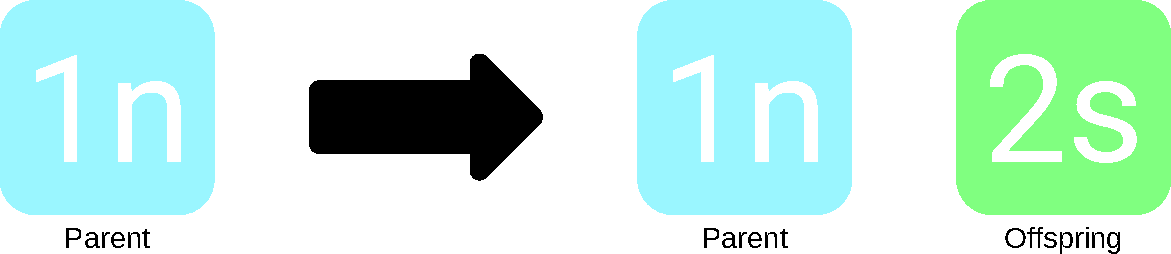
\includegraphics[width=\textwidth]{new_highchannel_offspring}\vspace{-10ex}}
\end{column}
\end{columns}
  \end{subfigure}
  \caption{
  Allowed multichannel inheritance outcomes;
  (\subref{fig:same_multichannel_offspring}) identical level 1 and 2 channels,
  (\subref{fig:new_lowchannel_offspring}) new level 1 channel with identical level 2 channel, and
  (\subref{fig:new_highchannel_offspring}) new level 1 and 2 channels.
  }
\end{figure}

\end{frame}

\begin{frame}{Multichannel Inheritance: Hierarchy}%
  \textbf{hierarchy explicitly enforced:}
  \begin{itemize}
    \item no option to generate offspring w/ new Level 1 channel and same Level 2 channel
    \item thus, same Level 1 channel $\rightarrow$ same Level 2 channel
  \end{itemize}

  \pause

  \vspace{2ex}
  \textbf{analogy:}
  \begin{itemize}
    \item citizens of the same province $\rightarrow$ citizens of same country
  \end{itemize}

\end{frame}

\begin{frame}{Outcome: Evolution of Level-two Individuality}
\begin{figure}
\begin{columns}
\begin{column}{0.6\textwidth}
\includegraphics<1>[width=\textwidth]{results/ChannelMap_1011_update0.png}%
\includegraphics<2>[width=\textwidth]{results/ChannelMap_1011_update500000.png}%
\includegraphics<3>[width=\textwidth]{results/ChannelMap_1011_update1000000.png}%
\includegraphics<4>[width=\textwidth]{results/ChannelMap_1011_update2000000.png}%
\includegraphics<5>[width=\textwidth]{results/ChannelMap_1011_update4000000.png}%
\includegraphics<6>[width=\textwidth]{results/ChannelMap_1011_update5000000.png}%
\includegraphics<7>[width=\textwidth]{results/ChannelMap_1011_update7000000.png}%
\end{column}
\begin{column}{0.4\textwidth}
\only<1>{Update: 0}%
\only<2>{Update: 500,000}%
\only<3>{Update: 1,000,000}%
\only<4>{Update: 2,000,000}%
\only<5>{Update: 4,000,000}%
\only<6>{Update: 5,000,000}%
\only<7>{Update: 7,000,000}%

\vspace{8ex}

\caption{Channel-map visualization of a simulation where second-level individuality evolved.}
\end{column}
\end{columns}
\end{figure}
\end{frame}

\begin{frame}{Future Work: Biologically-Motivated}

investigate roles of following w.r.t. major evolutionary transitions:
\pause
\begin{itemize}[<+->]
\item  pre-existing phenotypic plasticity \cite{clune2007investigating, lalejini2016evolutionary}
\item pre-existing environmental interactions
\item pre-existing reproductive division of labor
\end{itemize}

\end{frame}


\end{document}
